\documentclass[12pt,a4letter]{article}
%Các gói lệnh cơ bản
\usepackage{amsmath,amsxtra,amssymb,latexsym, amscd,amsthm}
\usepackage{indentfirst}
\usepackage[mathscr]{eucal}
\usepackage{graphicx}
\usepackage{makecell}
\usepackage{longtable}
\usepackage[utf8]{vietnam}
%Kích thước của trang đề thi
\voffset=-2cm
\hoffset=-2cm
\textheight 24truecm 
\textwidth 17truecm 
%Dùng gói lệnh cho câu hỏi và lời giải[nosolutionfiles]
\usepackage{answers}
\theoremstyle{definition}
\newtheorem{cauhoi}{Câu}
\Newassociation{traloi}{Soln}{goiytraloi}
\renewcommand{\Solnlabel}[1]{\textbf{Lời giải #1}.}

\newenvironment{phandiem}{%
\par\noindent
\begin{longtable}[t]{|p{15cm}|p{1.2cm}|}
\hline
}{%
\end{longtable}
}
\newcommand\diem[1]{ & \hfil \textbf{#1} \\ \hline}
\newcommand\tongdiem[1]{\hfill [\textbf{#1} điểm]}
%Định nghĩa tiêu đề
\def\tendhqg{\small \textbf{ĐẠI HỌC QUỐC GIA HÀ NỘI}}
\def\tentruong{\small \textbf{ĐẠI HỌC KHOA HỌC TỰ NHIÊN}}
\def\tenkythi{ĐỀ THI KẾT THÚC MÔN HỌC}
\def\namhoc{NĂM HỌC 2017-2018}
\def\tenmonhoc{TỐI ƯU HÓA}
\def\mamonhoc{MAT2407}
\def\sotinchi{3}
\def\svkhoa{K60}
\def\nganhhoc{MT\& KHMT, Toán - Tin ứng dụng}
\def\thoigian{90 phút }
\def\deso{2}
\def\dapan{ĐÁP ÁN VÀ THANG ĐIỂM}
\def\nguoilamdapan{PGS.TS. Nguyễn Hữu Điển}
\def\ngaylam{Hà nội, ngày 10 tháng 05 năm 2018}

\usepackage{mathpazo}
\usepackage{mathtools}
\usepackage{colortbl}
%%%%%%%%%%%%%%%%%%%%%%
\usepackage{arydshln}
\usepackage{multirow}
\newcommand{\gd}[1]{\multicolumn{1}{:c|}{#1}}
\newcommand{\gn}[1]{\cdashline{#1}}
\hdashlinewidth=8pt
%%%%%%%%%%%%%%%%%%%%%%
\graphicspath{{hinh/}}
\begin{document}
\setlength{\baselineskip}{16truept}
%Mở tệp ghi đáp án
\Opensolutionfile{goiytraloi}[traloi] 
%Phần tiêu đề của đề thi
\thispagestyle{empty}
\begin{minipage}[b]{0.4\textwidth}
\centering
\textbf{\tendhqg}\\
\textbf{\tentruong}\\ 
-------------\\
\quad \\
\end{minipage}
\hfill
\begin{minipage}[b]{0.6\textwidth}
\centering
\textbf{\tenkythi}\\
\textbf{ \namhoc}\\
------oOo-------\\ 
\qquad 
\end{minipage}

\centerline{\textbf{Môn thi:} \textbf{\tenmonhoc}}
\leftline{Mã môn học: \textbf{\mamonhoc}\ \hfil Số tín chỉ:  \textbf{\sotinchi} \hfil Đề số: \textbf{\deso} \hfil }
\leftline{Dành cho sinh viên khoá: \textbf{\svkhoa} \hfil Ngành học: \textbf{\nganhhoc}\hfil }
\centerline{Thời gian làm bài \textbf{\thoigian} (không kể thời gian phát đề)}
\noindent \hrulefill

%%%%%%%%%%%%%%%%%%%%%%%%%%%%%%%%%%%%
%Phần câu hỏi và trả lời
\begin{cauhoi}%1
(3 điểm)  
Cho bài toán quy hoạch tuyến tính
\begin{center}
$ L(x)=3x_1+4x_2+x_3\rightarrow\min $ \\
 $ \begin{dcases}
-3x_1+2x_2-4x_3&\ge 15\\ 
\phantom{-}2x_1-\phantom{2}x_2-5x_3&\ge 8\\ 
\phantom{-}4x_1+2x_2+2x_3&\ge 10\\ 
x_1, x_2\ge 0, x_3\le 0.&\\ 
\end{dcases} $
\end{center}
Cho biết bài toán trên có phương án tối ưu là $x^*=(7,0,-9)$.
Hãy lập và giải bài toán đối ngẫu của bài toán nói trên.

%%%%%%%%%%%%%%%%%%%%%%%Lời giải
\begin{traloi}\tongdiem{3}
\begin{phandiem}
Bài toán đối ngẫu của bài toán trên là
\begin{center}
$$g(x)=15y_1+8y_2+10y_3\rightarrow\max$$
$$\begin{cases}
-3y_1+2y_2+4y_3\le 3,&\\
2y_1-y_2+2y_3\le 4,&\\
-4y_1-5y_2+2y_3\ge 1,&\\
y_i\ge 0, i=\overline{1,3}.&
\end{cases}$$
\end{center}
\diem{1}
Do bài toán đã cho có phương án tối ưu là $x^*=(7,0,-9)$ nên theo định lý độ lệch bù yếu ta có hệ phương trình sau
$$\begin{cases}
y_2=0,&\\
-3y_1+2y_2+4y_3=3,&\\
-4y_1-5y_2+2y_3=1.&\\
\end{cases}$$
\diem{1}
Giải hệ phương trình trên ta được một nghiệm duy nhất là
$$y_1^*=\dfrac{1}{5}, y_2^*=0, y_3^*=\dfrac{9}{10}.$$
Nghiệm trên thỏa mãn các ràng buộc còn lại của bài toán đối ngẫu nên bài toán đối ngẫu có bài giảng tối ưu là $y^*=(\dfrac{1}{5},0,\dfrac{9}{10})$ và $g(y^*)=12$.
\diem{1}
\end{phandiem}
% \newpage
\end{traloi}
\end{cauhoi}


\begin{cauhoi}%2
(3 điểm)  
Cho bài toán quy hoạch tuyến tính
\begin{center}
$ L(x)=2x_1+4x_2-2x_3\rightarrow\min $ \\
 $ \begin{dcases}
\phantom{1}x_1-2x_2+\phantom{3}x_3&=27\\ 
2x_1+\phantom{2}x_2+2x_3&=50\\ 
\phantom{1}x_1-x_2-\phantom{3}x_3&\le 18\\ 
x_j\ge 0, j=1,2,3.&\\ 
\end{dcases} $
\end{center}

i) Đưa bài toán về dạng chính tắc;

ii) Giải bài toán bằng phương pháp đơn hình.

%%%%%%%%%%%%%%%%%Lời giải
\begin{traloi}
\tongdiem{3}
\begin{phandiem}
i) Thêm vào bài toán  ẩn phụ $x_4$ và hai ẩn giả $x_5, x_6$ dạng chính tắc tương đương:

\begin{center}
$ g(x)=2x_1+4x_2-2x_3+Mx_5+Mx_6\rightarrow\min $ \\
 $ \begin{dcases}
\phantom{1}x_1-2x_2+\phantom{3}x_3+x_5&=27\\ 
2x_1+\phantom{2}x_2+2x_3+x_6&=50\\ 
\phantom{1}x_1-x_2-\phantom{3}x_3+x_4&= 18\\ 
x_j\ge 0, j=1,2,3.&\\ 
\end{dcases} $
\end{center}
\diem{1}

 Giải bằng phương pháp đánh thuế: 
Bảng đơn hình
\begin{center}
\renewcommand{\arraystretch}{1.25}
\begin{tabular}{| l | l | l | l  l  l  l  l  l   |}
\hline
$J$&$c_J$&$x_J$&1&2&3&4&5&6\\ 
\cline{4-9}
   &     &   &2&4 &-2&0&M&M\\ 
\hline
5&M     & 27     &1 &-2      & 1      & 0& 1&0\\
6&M     & 50     &2 &1      & [2]      & 0& 0&1\\
4&0     &  18    & 1 &1      &   -1      & 1& 0&0\\
\hline
&M=0& 0 &-2 &-4 &2  &0& 0&0\\
&M=1&77& 3  &-1&[3]&0&0& 0\\
\hline
\end{tabular}
\end{center}
\diem{1}

Cột xoay $s=3$ và hàng xoay $r=6$:
\begin{center}
\renewcommand{\arraystretch}{1.25}
\begin{tabular}{| l | l | l | l  l  l  l  l  l   |}
\hline
$J$&$c_J$&$x_J$&1&2&3&4&5&6\\ 
\cline{4-9}
   &     &   &2&4 &-2&0&M&M\\ 
\hline
5&M     & 2     & 0 &-5/2      & 0      & 0& 1&\\
3&-2     & 25     &1 &1/2      & 1      & 0& 0&\\
4&0     &  43    & 2 &-1/2      & 0      & 1& 0&\\
\hline
&M=0&-50 &-4 &-5 &0  &0& 0&\\
&M=1& 2   & 0  &-5/2&0&0&0& \\
\hline
\end{tabular}
\end{center}

Trong bảng trên ta có $\Delta_j\le 0$ với mọi $j$, nên bài toán ở rộng có phương án tối ưu
$x^*=(0,0,25,43,2,0)$.

Do bài toán mở rộng có phương án tối ưu có ẩn giả $x^*_5=2>0$ nên bài toán ban đầu không có phương án tối ưu.
\diem{1}
\end{phandiem}
 \end{traloi}
\end{cauhoi}

\begin{cauhoi}%3
(4 điểm) Cho số liệu bài toán vận tải và ma trận cước phí $C$ như sau:

$a=(20, 45, 55)^T$, \qquad $b=(30, 25, 40, 25)^T$,
\quad
$C=\begin{bmatrix}
4&2&10&6\\ 
1&3&8&12\\ 
5&3&9&7\\ 
\end{bmatrix}$ 


a) Lập bảng vận tải cho bài toán trên.

b) Tìm phương án xuất phát theo phương pháp cước phí nhỏ nhất.

c) Giải bài toán vận tải trên theo phương pháp thế vị.

%%%%%%%%%%%%%%%%Lời giải
\begin{traloi}\tongdiem{4}\\
 \begin{phandiem}
\noindent 1. Kiểm tra điều kiện cân bằng của BTVT
\begin{center}
$\begin{aligned}
\sum\limits_{i=1}^{3}a_i&=20+45+55=120\\
\sum\limits_{j=1}^{4}b_j&=30+25+40+25=120
\end{aligned}$
\end{center}
\diem{0,25}
\noindent  2. Vòng lặp thứ nhất:

{\it Bước 1.} Tìm phương án xuất phát bằng phương pháp cực tiểu cước phí trong toàn bảng. Ta được phương án cực biên $x$ (xem bảng ~\ref{bang:ch407}).

% \begin{table}[!ht]
% \centering
%\input bang20092.tex
\begin{center}
\includegraphics[scale =1.2]{bang20092}
\end{center}
% \caption{Phương án đầu tiên }\label{bang:ch407}
% \end{table}
\diem{0,75}

{\it Bước 2.} Phương án $x$ không thoái hóa vì $|G|=m+n-1=6$. Tìm các thế vị cho $u_1=0$ suy ra 
\begin{center}
$\begin{aligned}
v_2&=c_{12}-u_1=2-0=2\\
u_2&=c_{22}-v_2=3-2=1\\
v_1&=c_{21}-u_2=1-1=0\\
v_3&=c_{23}-u_2=8-1=7\\
u_3&=c_{33}-v_3=9-7=2\\
v_4&=c_{34}-u_3=7-2=5
\end{aligned}$
\end{center}

{\it Bước 3.} Tính các ước lượng
\begin{center}
$\begin{aligned}
\Delta_{11}&=u_1+v_1-c_{11}=0+0-4=-4<0\\
\Delta_{13}&=u_1+v_3-c_{13}=0+7-10=-3<0\\
\Delta_{14}&=u_1+v_4-c_{14}=0+5-6=-1<0\\
\Delta_{24}&=u_2+v_2-c_{24}=1+5-12=-6<0\\
\Delta_{31}&=u_3+v_1-c_{31}=2+2-5=-1<0\\
\Delta_{32}&=u_3+v_2-c_{32}=2+2-3=1>0
\end{aligned}$
\end{center}

\diem{1}
{\it Bước 4.} $\Delta_{i' j'}=\Delta_{32}=1>0$ Ghép ô $(3,2)$ vào $G$ ta có chu trình
$$K: (2,2), (2,3), (3,3), (3,2)$$
Tương ứng với cách đánh dấu:  lẻ, chẵn, lẻ, chẵn.

{\it Bước 5.} Phá vỡ chu trình bằng cách lấy $\theta=\min \left\{ x_{i j}| (i, j)\in K\right\}=5$. Ta có 
bảng mới phương án $X'$:


% \begin{table}[!ht]
% \centering
%\input bang20093.tex
\begin{center}
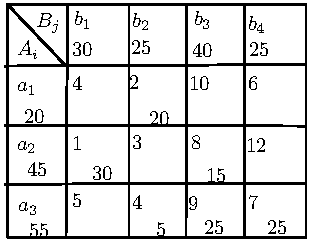
\includegraphics[scale =1.2]{bang20093}
\end{center}
% \caption{Bảng phương án mới}\label{bang:ch408}
% \end{table}

\diem{1}
\noindent 2. Vòng lặp thứ hai:

{\it Bước 1.} Đã xác định $X'$ như bảng trên.

{\it Bước 2.}  Thấy ngay $|G|=6$. Lấy $u_1=0$ suy ra
\begin{center}
$\begin{aligned}
v_2&=c_{12}-u_1=2-0=2\\
u_3&=c_{33}-v_2=3-2=1\\
v_3&=c_{33}-u_3=9-1=8\\
u_2&=c_{23}-v_3=8-8=0\\
v_1&=c_{21}-u_2=1-0=1\\
v_4&=c_{34}-u_3=7-1=6
\end{aligned}$
\end{center}

{\it Bước 3.} Tính các ước lượng
\begin{center}
$\begin{aligned}
\Delta_{11}&=u_1+v_1-c_{11}=0+1-4=-3<0\\
\Delta_{13}&=u_1+v_3-c_{13}=0+8-10=-2<0\\
\Delta_{14}&=u_1+v_4-c_{14}=0+6-6=0\\
\Delta_{22}&=u_2+v_2-c_{22}=0+2-3=-1<0\\
\Delta_{24}&=u_2+v_4-c_{24}=0+6-12=-6<0\\
\Delta_{31}&=u_3+v_1-c_{31}=1+1-5=-3<0
\end{aligned}$
\end{center}

Ta có phương án
$$x_{12}=20, x_{21}=30, x_{23}=15, x_{32}=5, x_{33}=25, x_{34}=25.$$
$$f_{\min}=20.2+1.30+8.15+3.5+9.25+7.25=605.$$
\diem{1}
 \end{phandiem}
\end{traloi}
\end{cauhoi}



%\noindent \hrulefill

%\textbf{Chú ý:} Cán bộ coi thi không giải thích gì thêm.
%%%%%%%%%%%%%%%%%%%%%%%%%%%%%%%%%%%%
%Phần đóng tệp đáp án và in ra
\Closesolutionfile{goiytraloi}
%%%%%%%%%%%%In đáp án
\newpage
\begin{center}
\textbf{\tendhqg} \\
\textbf{ \tentruong} \\                
 -----------------------\\
\textbf{\dapan}\\
\textbf{\tenkythi, \namhoc}\\
\centerline{\textbf{Môn thi:} \textbf{\tenmonhoc}}
\end{center}

\leftline{Mã môn học: \textbf{\mamonhoc}\ \hfil Số tín chỉ:  \textbf{\sotinchi} \hfil Đề số: \textbf{\deso} \hfil }
\leftline{Dành cho sinh viên khoá: \textbf{\svkhoa} \hfil Ngành học: \textbf{\nganhhoc}\hfil }

\small
\Readsolutionfile{goiytraloi}

\begin{flushright}
\parbox[c]{8cm}{\centering
\ngaylam\\
NGƯỜI LÀM ĐÁP ÁN\\
(ký và ghi rõ họ tên)\\

\vspace*{1.5cm}
\nguoilamdapan
}
\end{flushright}
\end{document}
 Nguyễn Thị Oanh 